\documentclass[tikz,border=10pt]{standalone}
\begin{document}
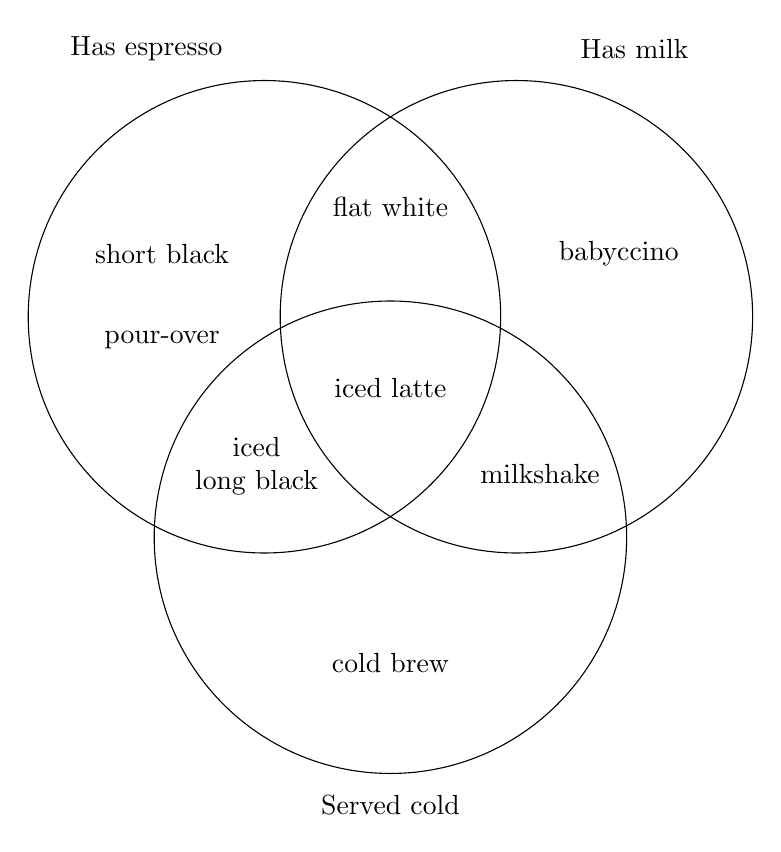
\begin{tikzpicture}
\draw (0,0) circle (3cm); \draw (3.2,0) circle (3cm); \draw (1.6,-2.8) circle (3cm);
\node at (-1.5,3.4) {Has espresso}; \node at (4.7,3.4) {Has milk}; \node at (1.6,-6.2) {Served cold};
\node at (-1.3,0.8) {short black};
\node at (4.5,0.8) {babyccino};
\node at (1.6,-4.4) {cold brew};
\node at (1.6,1.4) {flat white};
\node[align=center] at (-0.1,-1.9) {iced\\long black};
\node at (3.5,-2.0) {milkshake};
\node at (1.6,-0.9) {iced latte};
\node at (-1.3,-0.3) {pour-over};
\end{tikzpicture}
\end{document}
